\section{Экспериментальные методы}

\subsection{Атомно-силовая микроскопия}

В основе работы атомно-силового микроскопа (АСМ) лежит силовое взаимодействие между зондом и поверхностью, для регистрации которого используются специальные зондовые датчики, представляющие собой упругую консоль с острым зондом на конце (рисунок~\ref{fig:AFM}). Сила, действующая на зонд со стороны поверхности, приводит к изгибу консоли. Регистрируя величину изгиба, можно контролировать силу взаимодействия зонда с поверхностью.

Качественно работу АСМ можно пояснить на примере сил Ван-дер-Ваальса. Наиболее часто энергию ван-дер-ваальсова взаимодействия двух атомов, находящихся на расстоянии r друг от друга, аппроксимируют степенной функцией -- потенциалом Леннарда-Джонса:

\begin{equation}
	U_{LJ}(r)=U_0\left\{-2\left(\frac{r_0}{r}\right)^6+\left(\frac{r_0}{r}\right)^{12}\right\}.
\end{equation}
Первое слагаемое в данном выражении описывает дальнодействующее притяжение, обусловленное, в основном, диполь-дипольным взаимодействием атомов. Второе слагаемое учитывает отталкивание атомов на малых расстояниях. Параметр $r_0$ -- равновесное расстояние между атомами, $U_0$ -- значение энергии в минимуме.

\begin{figure}
	\centering
	\begin{minipage}{0.48\textwidth}
		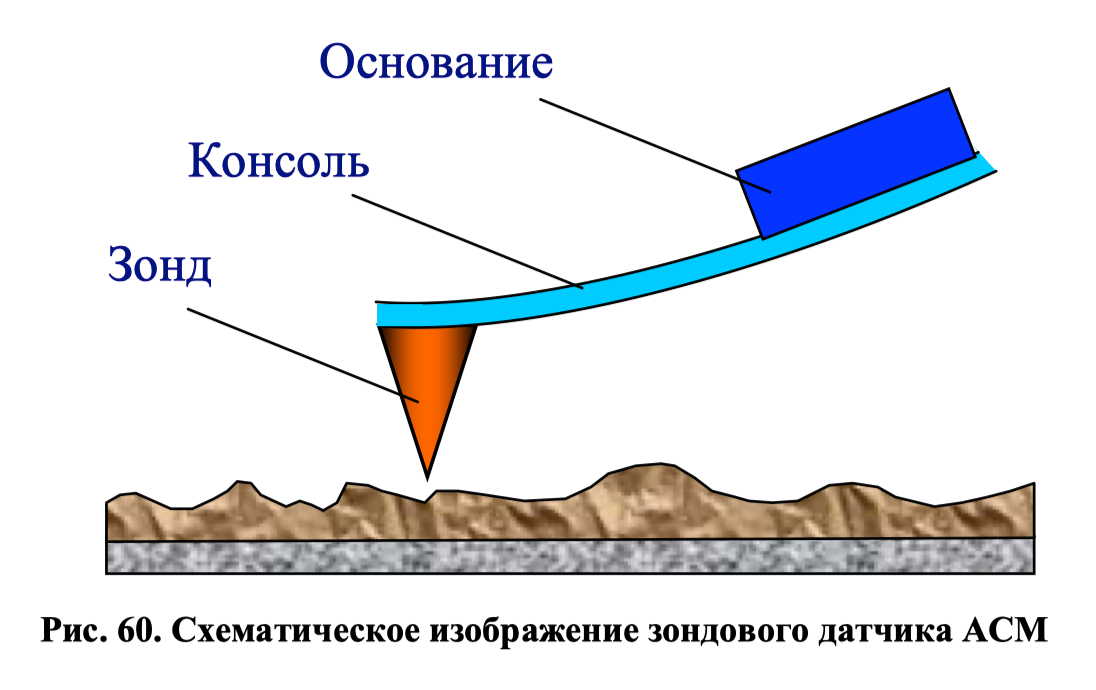
\includegraphics[width=0.9\textwidth]{AFM}
	\end{minipage}
	\begin{minipage}{0.48\textwidth}
		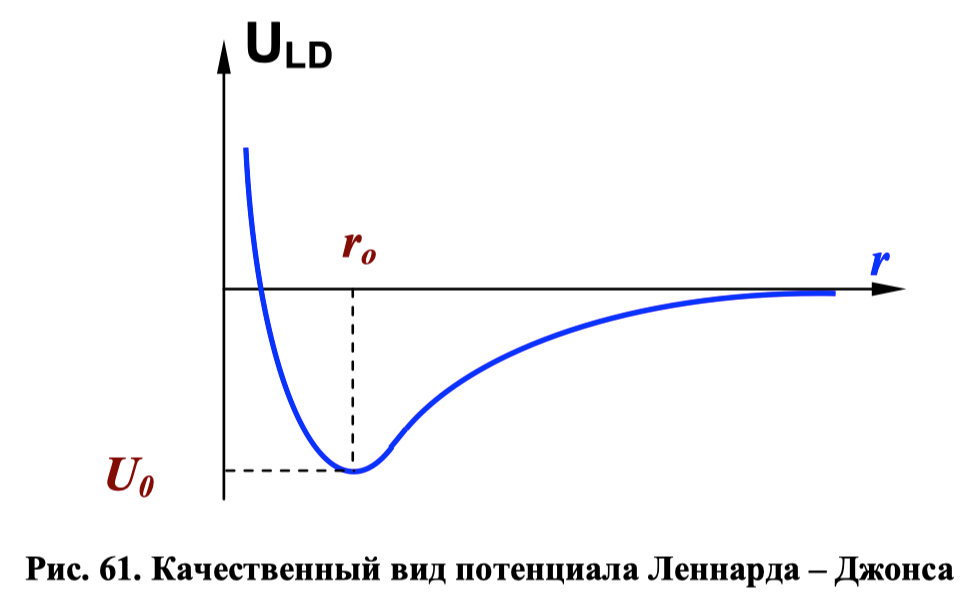
\includegraphics[width=0.9\textwidth]{LJ}
	\end{minipage}
	\caption{Схематическое изображение зондового датчика АСМ.}
	\label{fig:AFM}
\end{figure}

Потенциал Леннарда-Джонса позволяет оценить силу взаимодействия зонда с образцом [33]. Общую энергию системы можно получить, суммируя элементарные взаимодействия для каждого из атомов зонда и образца:
\begin{equation}
	W_{P S}=\iint_{V_P V_S} U_{L D}\left(r-r^{\prime}\right) n_P\left(r^{\prime}\right) n_S(r) d V d V^{\prime}
\end{equation}
где $n_S(r)$ и $n_P(r^\prime)$ -- плотности атомов в материале образца и зонда, соответственно. Соответственно сила, действующая на зонд со стороны поверхности, может быть вычислена следующим образом:
\begin{equation}
	\vec{F}_{P S}=-\operatorname{grad}\left(W_{P S}\right).
\end{equation}

В общем случае данная сила имеет как нормальную к поверхности, так и латеральную (лежащую в плоскости поверхности образца) составляющие. Реальное взаимодействие зонда с образцом имеет более сложный характер, однако основные черты данного взаимодействия сохраняются -- зонд АСМ испытывает притяжение со стороны образца на больших расстояниях и отталкивание на малых.

Получение АСМ изображений рельефа поверхности связано с регистрацией малых изгибов упругой консоли зондового датчика. В атомно-силовой микроскопии для этой цели широко используются оптические методы (рис.~\ref{fig:AFM_2}). Оптическая система АСМ юстируется таким образом, чтобы излучение полупроводникового лазера фокусировалось на консоли зондового датчика, а отраженный пучок попадал в центр фоточувствительной области фотоприемника. В качестве позиционно-чувствительных фотоприемников применяются четырехсекционные полупроводниковые фотодиоды.

\begin{figure}
	\centering
	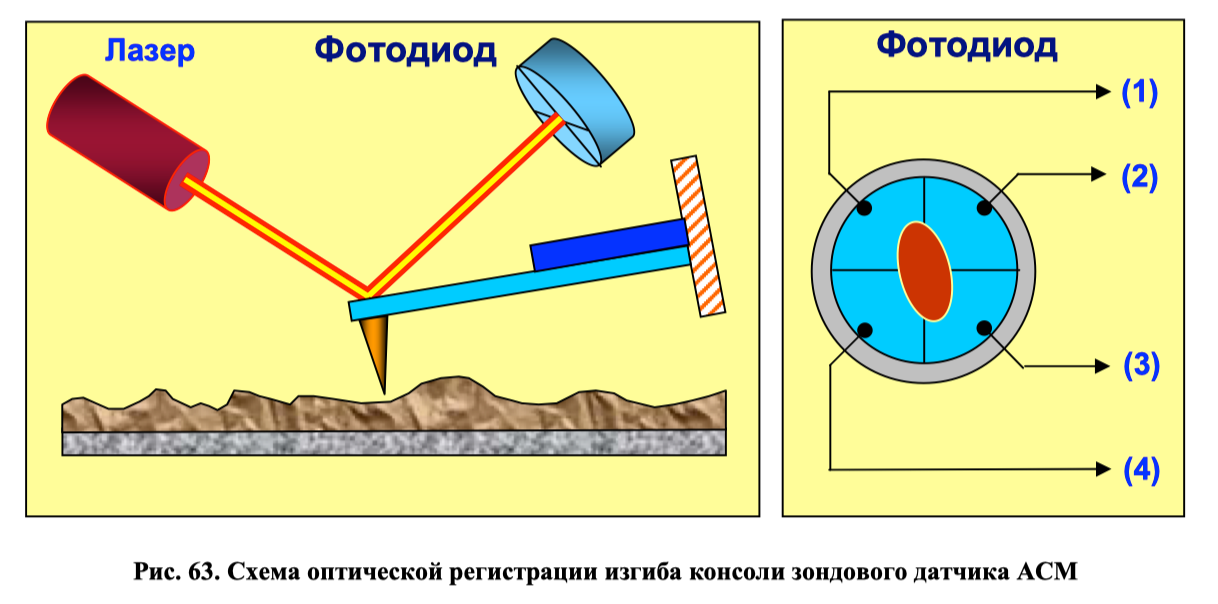
\includegraphics[width=0.9\textwidth]{AFM_2}
	\caption{Схематическое изображение зондового датчика АСМ.}
	\label{fig:AFM_2}
\end{figure}

Основные регистрируемые оптической системой параметры -- это деформации изгиба консоли под действием $Z$-компонент сил притяжения или отталкивания ($F_Z$) и деформации кручения консоли под действием латеральных компонент сил ($F_L$) взаимодействия зонда с поверхностью. Если обозначить исходные значения фототока в секциях фотодиода через $I_{01}$, $I_{02}$, $I_{03}$, $I_{04}$, а через $I_{1}$, $I_{2}$, $I_{3}$, $I_{4}$ -- значения токов после изменения положения консоли, то разностные токи с различных секций фотодиода $\Delta I_i = I_i - I_{0i}$ будут однозначно характеризовать величину и направление изгиба консоли зондового датчика АСМ. Действительно, комбинация разностных токов вида
\begin{equation}
	\Delta I_Z = \left(\Delta I_1+\Delta I_2\right)-\left(\Delta I_3+\Delta I_4\right)
\end{equation}
пропорциональна изгибу консоли под действием силы, действующей по нормали к поверхности образца, а комбинация разностных токов вида
\begin{equation}
	\Delta I_L=\left(\Delta I_1+\Delta I_4\right)-\left(\Delta I_2+\Delta I_3\right)
\end{equation}
характеризует изгиб консоли под действием латеральных сил.

Величина $\Delta I_Z$ используется в качестве входного параметра в петле обратной связи атомно-силового микроскопа. Система обратной связи обеспечивает постоянное значение $\Delta I_Z$ с помощью пьезоэлектрического исполнительного элемента, который поддерживает изгиб консоли $\Delta Z$ равным величине $\Delta Z_0$, задаваемой оператором.

При сканировании образца в режиме $\Delta Z = const$ зонд перемещается вдоль поверхности, при этом напряжение на $Z$-электроде сканера записывается в память компьютера в качестве рельефа поверхности $Z = f(X, Y)$. Пространственное разрешение АСМ определяется радиусом закругления зонда и чувствительностью системы, регистрирующей отклонения консоли. В настоящее время реализованы конструкции АСМ, позволяющие получать атомарное разрешение при исследовании поверхности образцов.